%!TeX root=../houndtop.tex
\chapter{Three Broken Threads}
\lettrine[lines=1]{S}{herlock} Holmes had, in a very remarkable degree, the power of detaching his mind at will. For two hours the strange business in which we had been involved appeared to be forgotten, and he was entirely absorbed in the pictures of the modern Belgian masters. He would talk of nothing but art, of which he had the crudest ideas, from our leaving the gallery until we found ourselves at the Northumberland Hotel.

»Sir Henry Baskerville is upstairs expecting you,« said the clerk. »He asked me to show you up at once when you came.«

»Have you any objection to my looking at your register?« said Holmes.

»Not in the least.«

The book showed that two names had been added after that of Baskerville. One was Theophilus Johnson and family, of Newcastle; the other Mrs Oldmore and maid, of High Lodge, Alton.

»Surely that must be the same Johnson whom I used to know,« said Holmes to the porter. »A lawyer, is he not, gray-headed, and walks with a limp?«

»No, sir; this is Mr Johnson, the coal-owner, a very active gentleman, not older than yourself.«

»Surely you are mistaken about his trade?«

»No, sir! he has used this hotel for many years, and he is very well known to us.«

»Ah, that settles it. Mrs Oldmore, too; I seem to remember the name. Excuse my curiosity, but often in calling upon one friend one finds another.«

»She is an invalid lady, sir. Her husband was once mayor of Gloucester. She always comes to us when she is in town.«

»Thank you; I am afraid I cannot claim her acquaintance. We have established a most important fact by these questions, Watson,« he continued in a low voice as we went upstairs together. »We know now that the people who are so interested in our friend have not settled down in his own hotel. That means that while they are, as we have seen, very anxious to watch him, they are equally anxious that he should not see them. Now, this is a most suggestive fact.«

»What does it suggest?«

»It suggests\allowbreak---\allowbreak halloa, my dear fellow, what on earth is the matter?«

As we came round the top of the stairs we had run up against Sir Henry Baskerville himself. His face was flushed with anger, and he held an old and dusty boot in one of his hands. So furious was he that he was hardly articulate, and when he did speak it was in a much broader and more Western dialect than any which we had heard from him in the morning.

»Seems to me they are playing me for a sucker in this hotel,« he cried. »They'll find they've started in to monkey with the wrong man unless they are careful. By thunder, if that chap can't find my missing boot there will be trouble. I can take a joke with the best, Mr Holmes, but they've got a bit over the mark this time.«

»Still looking for your boot?«

»Yes, sir, and mean to find it.«

»But, surely, you said that it was a new brown boot?«

»So it was, sir. And now it's an old black one.«

»What! you don't mean to say\allowbreak---\allowbreak ?«

»That's just what I do mean to say. I only had three pairs in the world\allowbreak---\allowbreak the new brown, the old black, and the patent leathers, which I am wearing. Last night they took one of my brown ones, and to-day they have sneaked one of the black. Well, have you got it? Speak out, man, and don't stand staring!«

An agitated German waiter had appeared upon the scene.

»No, sir; I have made inquiry all over the hotel, but I can hear no word of it.«

»Well, either that boot comes back before sundown or I'll see the manager and tell him that I go right straight out of this hotel.«

»It shall be found, sir\allowbreak---\allowbreak I promise you that if you will have a little patience it will be found.«

»Mind it is, for it's the last thing of mine that I'll lose in this den of thieves. Well, well, Mr Holmes, you'll excuse my troubling you about such a trifle\longdash«

»I think it's well worth troubling about.«

»Why, you look very serious over it.«

»How do you explain it?«

»I just don't attempt to explain it. It seems the very maddest, queerest thing that ever happened to me.«

»The queerest perhaps\longdash« said Holmes, thoughtfully.

»What do you make of it yourself?«

»Well, I don't profess to understand it yet. This case of yours is very complex, Sir Henry. When taken in conjunction with your uncle's death I am not sure that of all the five hundred cases of capital importance which I have handled there is one which cuts so deep. But we hold several threads in our hands, and the odds are that one or other of them guides us to the truth. We may waste time in following the wrong one, but sooner or later we must come upon the right.«

We had a pleasant luncheon in which little was said of the business which had brought us together. It was in the private sitting-room to which we afterwards repaired that Holmes asked Baskerville what were his intentions.

»To go to Baskerville Hall.«

»And when?«

»At the end of the week.«

»On the whole,« said Holmes, »I think that your decision is a wise one. I have ample evidence that you are being dogged in London, and amid the millions of this great city it is difficult to discover who these people are or what their object can be. If their intentions are evil they might do you a mischief, and we should be powerless to prevent it. You did not know, Dr Mortimer, that you were followed this morning from my house?«

Dr Mortimer started violently.

»Followed! By whom?«

»That, unfortunately, is what I cannot tell you. Have you among your neighbours or acquaintances on Dartmoor any man with a black, full beard?«

»No\allowbreak---\allowbreak or, let me see\allowbreak---\allowbreak why, yes. Barrymore, Sir Charles's butler, is a man with a full, black beard.«

»Ha! Where is Barrymore?«

»He is in charge of the Hall.«

»We had best ascertain if he is really there, or if by any possibility he might be in London.«

»How can you do that?«

»Give me a telegraph form. »Is all ready for Sir Henry?« That will do. Address to Mr Barrymore, Baskerville Hall. What is the nearest telegraph-office? Grimpen. Very good, we will send a second wire to the postmaster, Grimpen: »Telegram to Mr Barrymore to be delivered into his own hand. If absent, please return wire to Sir Henry Baskerville, Northumberland Hotel.« That should let us know before evening whether Barrymore is at his post in Devonshire or not.«

»That's so,« said Baskerville. »By the way, Dr Mortimer, who is this Barrymore, anyhow?«

»He is the son of the old caretaker, who is dead. They have looked after the Hall for four generations now. So far as I know, he and his wife are as respectable a couple as any in the county.«

»At the same time,« said Baskerville, »it's clear enough that so long as there are none of the family at the Hall these people have a mighty fine home and nothing to do.«

»That is true.«

»Did Barrymore profit at all by Sir Charles's will?« asked Holmes.

»He and his wife had five hundred pounds\footnote{Approximately \pounds 53,000 in 2023.} each.«

»Ha! Did they know that they would receive this?«

»Yes; Sir Charles was very fond of talking about the provisions of his will.«

»That is very interesting.«

»I hope,« said Dr Mortimer, »that you do not look with suspicious eyes upon everyone who received a legacy from Sir Charles, for I also had a thousand pounds\footnote{Approximately \pounds 106,000 in 2023.} left to me.«

»Indeed! And anyone else?«

»There were many insignificant sums to individuals, and a large number of public charities. The residue all went to Sir Henry.«

»And how much was the residue?«

»Seven hundred and forty thousand pounds.\footnote{Over \pounds 78 million in 2023.}«

Holmes raised his eyebrows in surprise. »I had no idea that so gigantic a sum was involved,« said he.

»Sir Charles had the reputation of being rich, but we did not know how very rich he was until we came to examine his securities. The total value of the estate was close on to a million.«

»Dear me! It is a stake for which a man might well play a desperate game. And one more question, Dr Mortimer. Supposing that anything happened to our young friend here\allowbreak---\allowbreak you will forgive the unpleasant hypothesis!\allowbreak---\allowbreak who would inherit the estate?«

»Since Rodger Baskerville, Sir Charles's younger brother died unmarried, the estate would descend to the Desmonds, who are distant cousins. James Desmond is an elderly clergyman in Westmoreland.«

»Thank you. These details are all of great interest. Have you met Mr James Desmond?«

»Yes; he once came down to visit Sir Charles. He is a man of venerable appearance and of saintly life. I remember that he refused to accept any settlement from Sir Charles, though he pressed it upon him.«

»And this man of simple tastes would be the heir to Sir Charles's thousands.«

»He would be the heir to the estate because that is entailed. He would also be the heir to the money unless it were willed otherwise by the present owner, who can, of course, do what he likes with it.«

»And have you made your will, Sir Henry?«

»No, Mr Holmes, I have not. I've had no time, for it was only yesterday that I learned how matters stood. But in any case I feel that the money should go with the title and estate. That was my poor uncle's idea. How is the owner going to restore the glories of the Baskervilles if he has not money enough to keep up the property? House, land, and dollars must go together.«

»Quite so. Well, Sir Henry, I am of one mind with you as to the advisability of your going down to Devonshire without delay. There is only one provision which I must make. You certainly must not go alone.«

»Dr Mortimer returns with me.«


\begin{figure}[t!h]
\centering

\includegraphics[width=.8\linewidth]{05_proposition}
\caption{The proposition took me completely by surprise}
\end{figure}
%\afterpage{\clearpage}

»But Dr Mortimer has his practice to attend to, and his house is miles away from yours. With all the good will in the world he may be unable to help you. No, Sir Henry, you must take with you someone, a trusty man, who will be always by your side.«

»Is it possible that you could come yourself, Mr Holmes?«

»If matters came to a crisis I should endeavour to be present in person; but you can understand that, with my extensive consulting practice and with the constant appeals which reach me from many quarters, it is impossible for me to be absent from London for an indefinite time. At the present instant one of the most revered names in England is being besmirched by a blackmailer, and only I can stop a disastrous scandal. You will see how impossible it is for me to go to Dartmoor.«

»Whom would you recommend, then?«

Holmes laid his hand upon my arm.

»If my friend would undertake it there is no man who is better worth having at your side when you are in a tight place. No one can say so more confidently than I.«

The proposition took me completely by surprise, but before I had time to answer, Baskerville seized me by the hand and wrung it heartily.

»Well, now, that is real kind of you, Dr Watson,« said he. »You see how it is with me, and you know just as much about the matter as I do. If you will come down to Baskerville Hall and see me through I'll never forget it.«

The promise of adventure had always a fascination for me, and I was complimented by the words of Holmes and by the eagerness with which the baronet hailed me as a companion.

»I will come, with pleasure,« said I. »I do not know how I could employ my time better.«

»And you will report very carefully to me,« said Holmes. »When a crisis comes, as it will do, I will direct how you shall act. I suppose that by Saturday all might be ready?«

»Would that suit Dr Watson?«

»Perfectly.«

»Then on Saturday, unless you hear to the contrary, we shall meet at the 10:30 train from Paddington.«

We had risen to depart when Baskerville gave a cry, of triumph, and diving into one of the corners of the room he drew a brown boot from under a cabinet.

»My missing boot!« he cried.

»May all our difficulties vanish as easily!« said Sherlock Holmes.

»But it is a very singular thing,« Dr Mortimer remarked. »I searched this room carefully before lunch.«

»And so did I,« said Baskerville. »Every inch of it.«

»There was certainly no boot in it then.«

»In that case the waiter must have placed it there while we were lunching.«

The German was sent for but professed to know nothing of the matter, nor could any inquiry clear it up. Another item had been added to that constant and apparently purposeless series of small mysteries which had succeeded each other so rapidly. Setting aside the whole grim story of Sir Charles's death, we had a line of inexplicable incidents all within the limits of two days, which included the receipt of the printed letter, the black-bearded spy in the hansom, the loss of the new brown boot, the loss of the old black boot, and now the return of the new brown boot. Holmes sat in silence in the cab as we drove back to Baker Street, and I knew from his drawn brows and keen face that his mind, like my own, was busy in endeavouring to frame some scheme into which all these strange and apparently disconnected episodes could be fitted. All afternoon and late into the evening he sat lost in tobacco and thought.

Just before dinner two telegrams were handed in. The first ran:
\begin{samepage}
\blockquote{
\textsc{Have just heard that Barrymore is at the Hall.}
\begin{flushright}
\allowbreak---\allowbreak  {\small\scshape BASKERVILLE.}
\end{flushright} 
}
\end{samepage}

The second:
\begin{samepage}
\blockquote{
\textsc{Visited twenty-three hotels as directed, but sorry, to report unable to trace cut sheet of Times.}
\begin{flushright}
\allowbreak---\allowbreak  {\small\scshape CARTWRIGHT.}
\end{flushright}
}
\end{samepage}

»There go two of my threads, Watson. There is nothing more stimulating than a case where everything goes against you. We must cast round for another scent.«

»We have still the cabman who drove the spy.«

»Exactly. I have wired to get his name and address from the Official Registry. I should not be surprised if this were an answer to my question.«

The ring at the bell proved to be something even more satisfactory than an answer, however, for the door opened and a rough-looking fellow entered who was evidently the man himself.

»I got a message from the head office that a gent at this address had been inquiring for 2704,« said he. »I've driven my cab this seven years and never a word of complaint. I came here straight from the Yard to ask you to your face what you had against me.«

»I have nothing in the world against you, my good man,« said Holmes. »On the contrary, I have half a sovereign for you if you will give me a clear answer to my questions.«

»Well, I've had a good day and no mistake,« said the cabman, with a grin. »What was it you wanted to ask, sir?«

»First of all your name and address, in case I want you again.«

»John Clayton, 3 Turpey Street, the Borough. My cab is out of Shipley's Yard, near Waterloo Station.«

Sherlock Holmes made a note of it.

»Now, Clayton, tell me all about the fare who came and watched this house at ten o'clock this morning and afterwards followed the two gentlemen down Regent Street.«

The man looked surprised and a little embarrassed. »Why, there's no good my telling you things, for you seem to know as much as I do already,« said he. »The truth is that the gentleman told me that he was a detective and that I was to say nothing about him to anyone.«

»My good fellow, this is a very serious business, and you may find yourself in a pretty bad position if you try to hide anything from me. You say that your fare told you that he was a detective?«

»Yes, he did.«

»When did he say this?«

»When he left me.«

»Did he say anything more?«

»He mentioned his name.«


Holmes cast a swift glance of triumph at me. »Oh, he mentioned his name, did he? That was imprudent. What was the name that he mentioned?«

»His name,« said the cabman, »was Mr Sherlock Holmes.«

Never have I seen my friend more completely taken aback than by the cabman's reply. For an instant he sat in silent amazement. Then he burst into a hearty laugh.

»A touch, Watson\allowbreak---\allowbreak an undeniable touch!« said he. »I feel a foil as quick and supple as my own. He got home upon me very prettily that time. So his name was Sherlock Holmes, was it?«

»Yes, sir, that was the gentleman's name.«

»Excellent! Tell me where you picked him up and all that occurred.«

»He hailed me at half-past nine in Trafalgar Square. He said that he was a detective, and he offered me two guineas if I would do exactly what he wanted all day and ask no questions. I was glad enough to agree. First we drove down to the Northumberland Hotel and waited there until two gentlemen came out and took a cab from the rank. We followed their cab until it pulled up somewhere near here.«

»This very door,« said Holmes.

»Well, I couldn't be sure of that, but I dare say my fare knew all about it. We pulled up half-way down the street and waited an hour and a half. Then the two gentlemen passed us, walking, and we followed down Baker Street and along\longdash«

»I know,« said Holmes.

»Until we got three-quarters down Regent Street. Then my gentleman threw up the trap, and he cried that I should drive right away to Waterloo Station as hard as I could go. I whipped up the mare and we were there under the ten minutes. Then he paid up his two guineas, like a good one, and away he went into the station. Only just as he was leaving he turned round and he said: »It might interest you to know that you have been driving Mr Sherlock Holmes.« That's how I come to know the name.«

»I see. And you saw no more of him?«

\begin{figure}[tbhp]
\centering

\includegraphics[width=0.7\textwidth]{05_cabman}
\caption{His name was »Mr Sherlock Holmes«.}
\end{figure}

\afterpage{\clearpage}


»Not after he went into the station.«

»And how would you describe Mr Sherlock Holmes?«

The cabman scratched his head. »Well, he wasn't altogether such an easy gentleman to describe. I'd put him at forty years of age, and he was of a middle height, two or three inches shorter than you, sir. He was dressed like a toff, and he had a black beard, cut square at the end, and a pale face. I don't know as I could say more than that.«

»Colour of his eyes?«

»No, I can't say that.«

»Nothing more that you can remember?«

»No, sir; nothing.«

»Well, then, here is your half-sovereign. There's another one waiting for you if you can bring any more information. Good night!«

»Good night, sir, and thank you!«

John Clayton departed chuckling, and Holmes turned to me with a shrug of his shoulders and a rueful smile.

»Snap goes our third thread, and we end where we began,« said he. »The cunning rascal! He knew our number, knew that Sir Henry Baskerville had consulted me, spotted who I was in Regent Street, conjectured that I had got the number of the cab and would lay my hands on the driver, and so sent back this audacious message. I tell you, Watson, this time we have got a foeman who is worthy of our steel. I've been checkmated in London. I can only wish you better luck in Devonshire. But I'm not easy in my mind about it.«

»About what?«

»About sending you. It's an ugly business, Watson, an ugly dangerous business, and the more I see of it the less I like it. Yes, my dear fellow, you may laugh, but I give you my word that I shall be very glad to have you back safe and sound in Baker Street once more.«
\clearpage
\vfill
\begin{figure}[hp!]
\centering
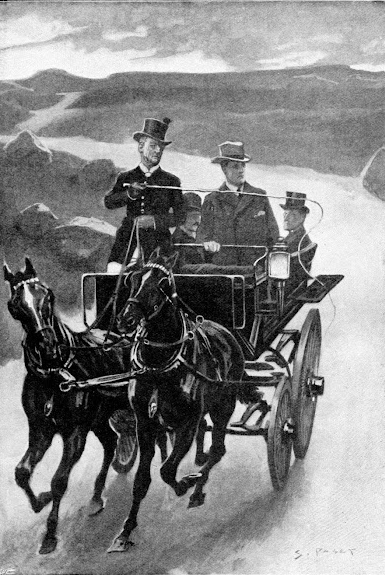
\includegraphics[width=\textwidth]{06_driverwhip}
\caption{The driver pointed with his whip—»Baskerville Hall,« said he.}
\end{figure}
\vfill
\thispagestyle{empty}
\clearpage
